The Brocard points $\Omega_1,\Omega_2$, shown in Figure~\ref{fig:brocard-basic} are well-studied, unique points of concurrence in a triangle, introduced by August L. Crelle in 1816, given a construction by Karl F.A. Jacobi in 1825, and rediscovered by Henri Brocard in 1875 \cite[Brocard Points]{mw}. 

\begin{figure}
    \centering
    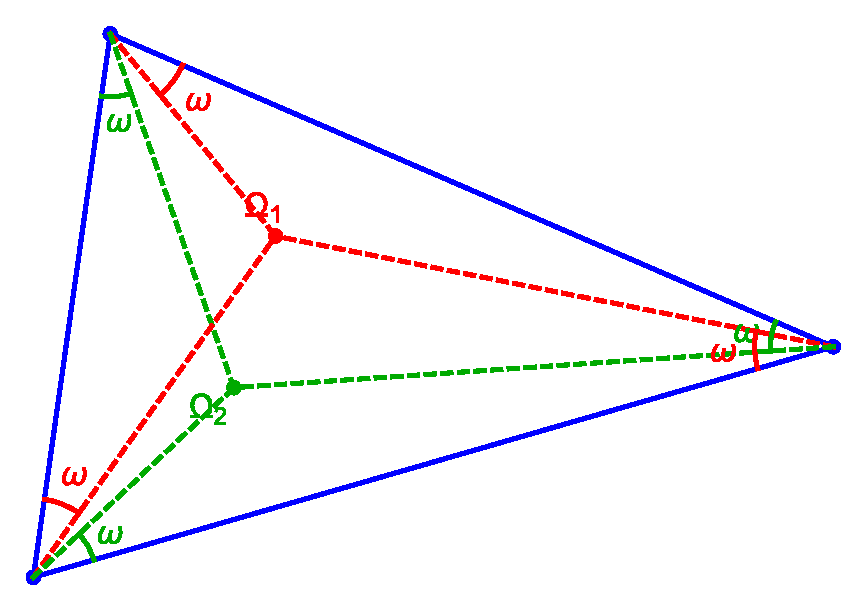
\includegraphics[width=.7\textwidth]{pics_06_0010_brocard_basic_single.eps}
    \caption{The Brocard Points $\Omega_1$ (resp. $\Omega_2$) are where sides of a triangle concur when rotated about each vertex by the Brocard angle $\omega$. When sides are traversed and rotated clockwise (resp. counterclockwise), one obtains $\Omega_1$ (resp. $\Omega_2$).}
    \label{fig:brocard-basic}
\end{figure}

The concept of a ``porism'', referred to below, is illustrated with one named after Poncelet  \cite{dragovic11}: given two conics $\Cm_1$ and $\Cm_2$, a 1d family of N-sided polygons inscribed in $\Cm_1$ while simultaneously circumscribing $\Cm_2$ can be constructed departing from either (i) all points on $\Cm_1$ or (ii) no point on $\Cm_1$, i.e., a ``porism'' is a mathematical statement which is either true everywhere or nowhere.

A special type of Poncelet porism is the ``Brocard porism'' \cite{bradley2007-brocard}: a 1d family of Poncelet 3-gons (triangles) inscribed in a circle and circumscribed about an ellipse $\E$ known as the {\em Brocard Inellipse}; see Figure~\ref{fig:broc-por-sec-tri}. Remarkably, the Brocard angle $\omega$ is invariant {\em and} the Brocard points $\Omega_1$ and $\Omega_2$ are stationary at the foci of $\E$.

As shorthand, below we refer to notable points of a triangle using Kimberling's notation $X_k$ \cite{etc}. For example, $X_1$ (resp. $X_2$, $X_3$, etc.) is the incenter (resp. barycenter, circumcenter, etc.).

As a review, the circle $\K$ which contains both Brocard points and the circumcenter $X_3$ is known as the Brocard {\em circle} \cite{mw}. Since over the porism all said points are stationary, so is $\K$. A lesser-known and property-rich point of the triangle is its Symmedian point $X_6$, where reflections of medians on angle bisectors concur \cite{etc}. It turns out $X_6$ is antipodal to $X_3$ on $\K$ and is therefore over the family it is motionless (stationary). $X_3$ and $X_6$ both lie  on the Brocard {\em axis} and $\K$ is centered on their midpoint $X_{182}$.

A full eight Brocard {\em triangles}
%\footnote{The 7th and 8th Brocard triangles were conceived during this research.}
have been classified (named 1st, 2nd, etc.) \cite{gibert2020-brocard}, deriving directly from $\Omega_{1,2},\K$ and related objects. It turns out the 1st, 2nd, and 7th Brocard triangles are inscribed in $\K$; see this \href{http://youtu.be/_bK-BCQv24A}{Video}.

Over the Brocard porism, amongst all the 8 Brocard triangles, only the 2nd and 5th Brocard triangles maintain stationary Brocard points; see Figure~\ref{fig:iteration}, this \href{https://bit.ly/2SG7Dxr}{animation} and this \href{https://youtu.be/MprJtB4UW9s}{Video}. Since  the 5th is homothetic to the reference (at $X_{32}$ \cite{gibert2020-anti-brocard}) we deem it less interesting. We focus on properties of the {\em second} Brocard triangle $T'$ whose vertices lie at the intersections of symmedians (cevians through the symmedian point $X_6$) with $\K$ \cite[Second Brocard Triangle]{mw}; see Figure~\ref{fig:broc-por-sec-tri}.

\subsection*{Main results}

Below the {\em isodynamic points} $X_{15}$ and $X_{16}$ of a triangle are mentioned, studied by J. Neuberg in the 1880s. These are the two common intersections of three special circles\footnote{Consider a triangle $T=ABC$. A first circle passes through (i) $A$, (ii) the intersection of the $A$-bisector with the opposite side $BC$, and (iii) the intersection of the $A$-external bisector with $BC$. The other two circles are constructed cyclically. It turns out these 3 circles intersect on two points only.} derived from a triangle, see \href{https://en.wikipedia.org/wiki/Isodynamic_point}{this page} for the construction.

\begin{figure}
    \centering
    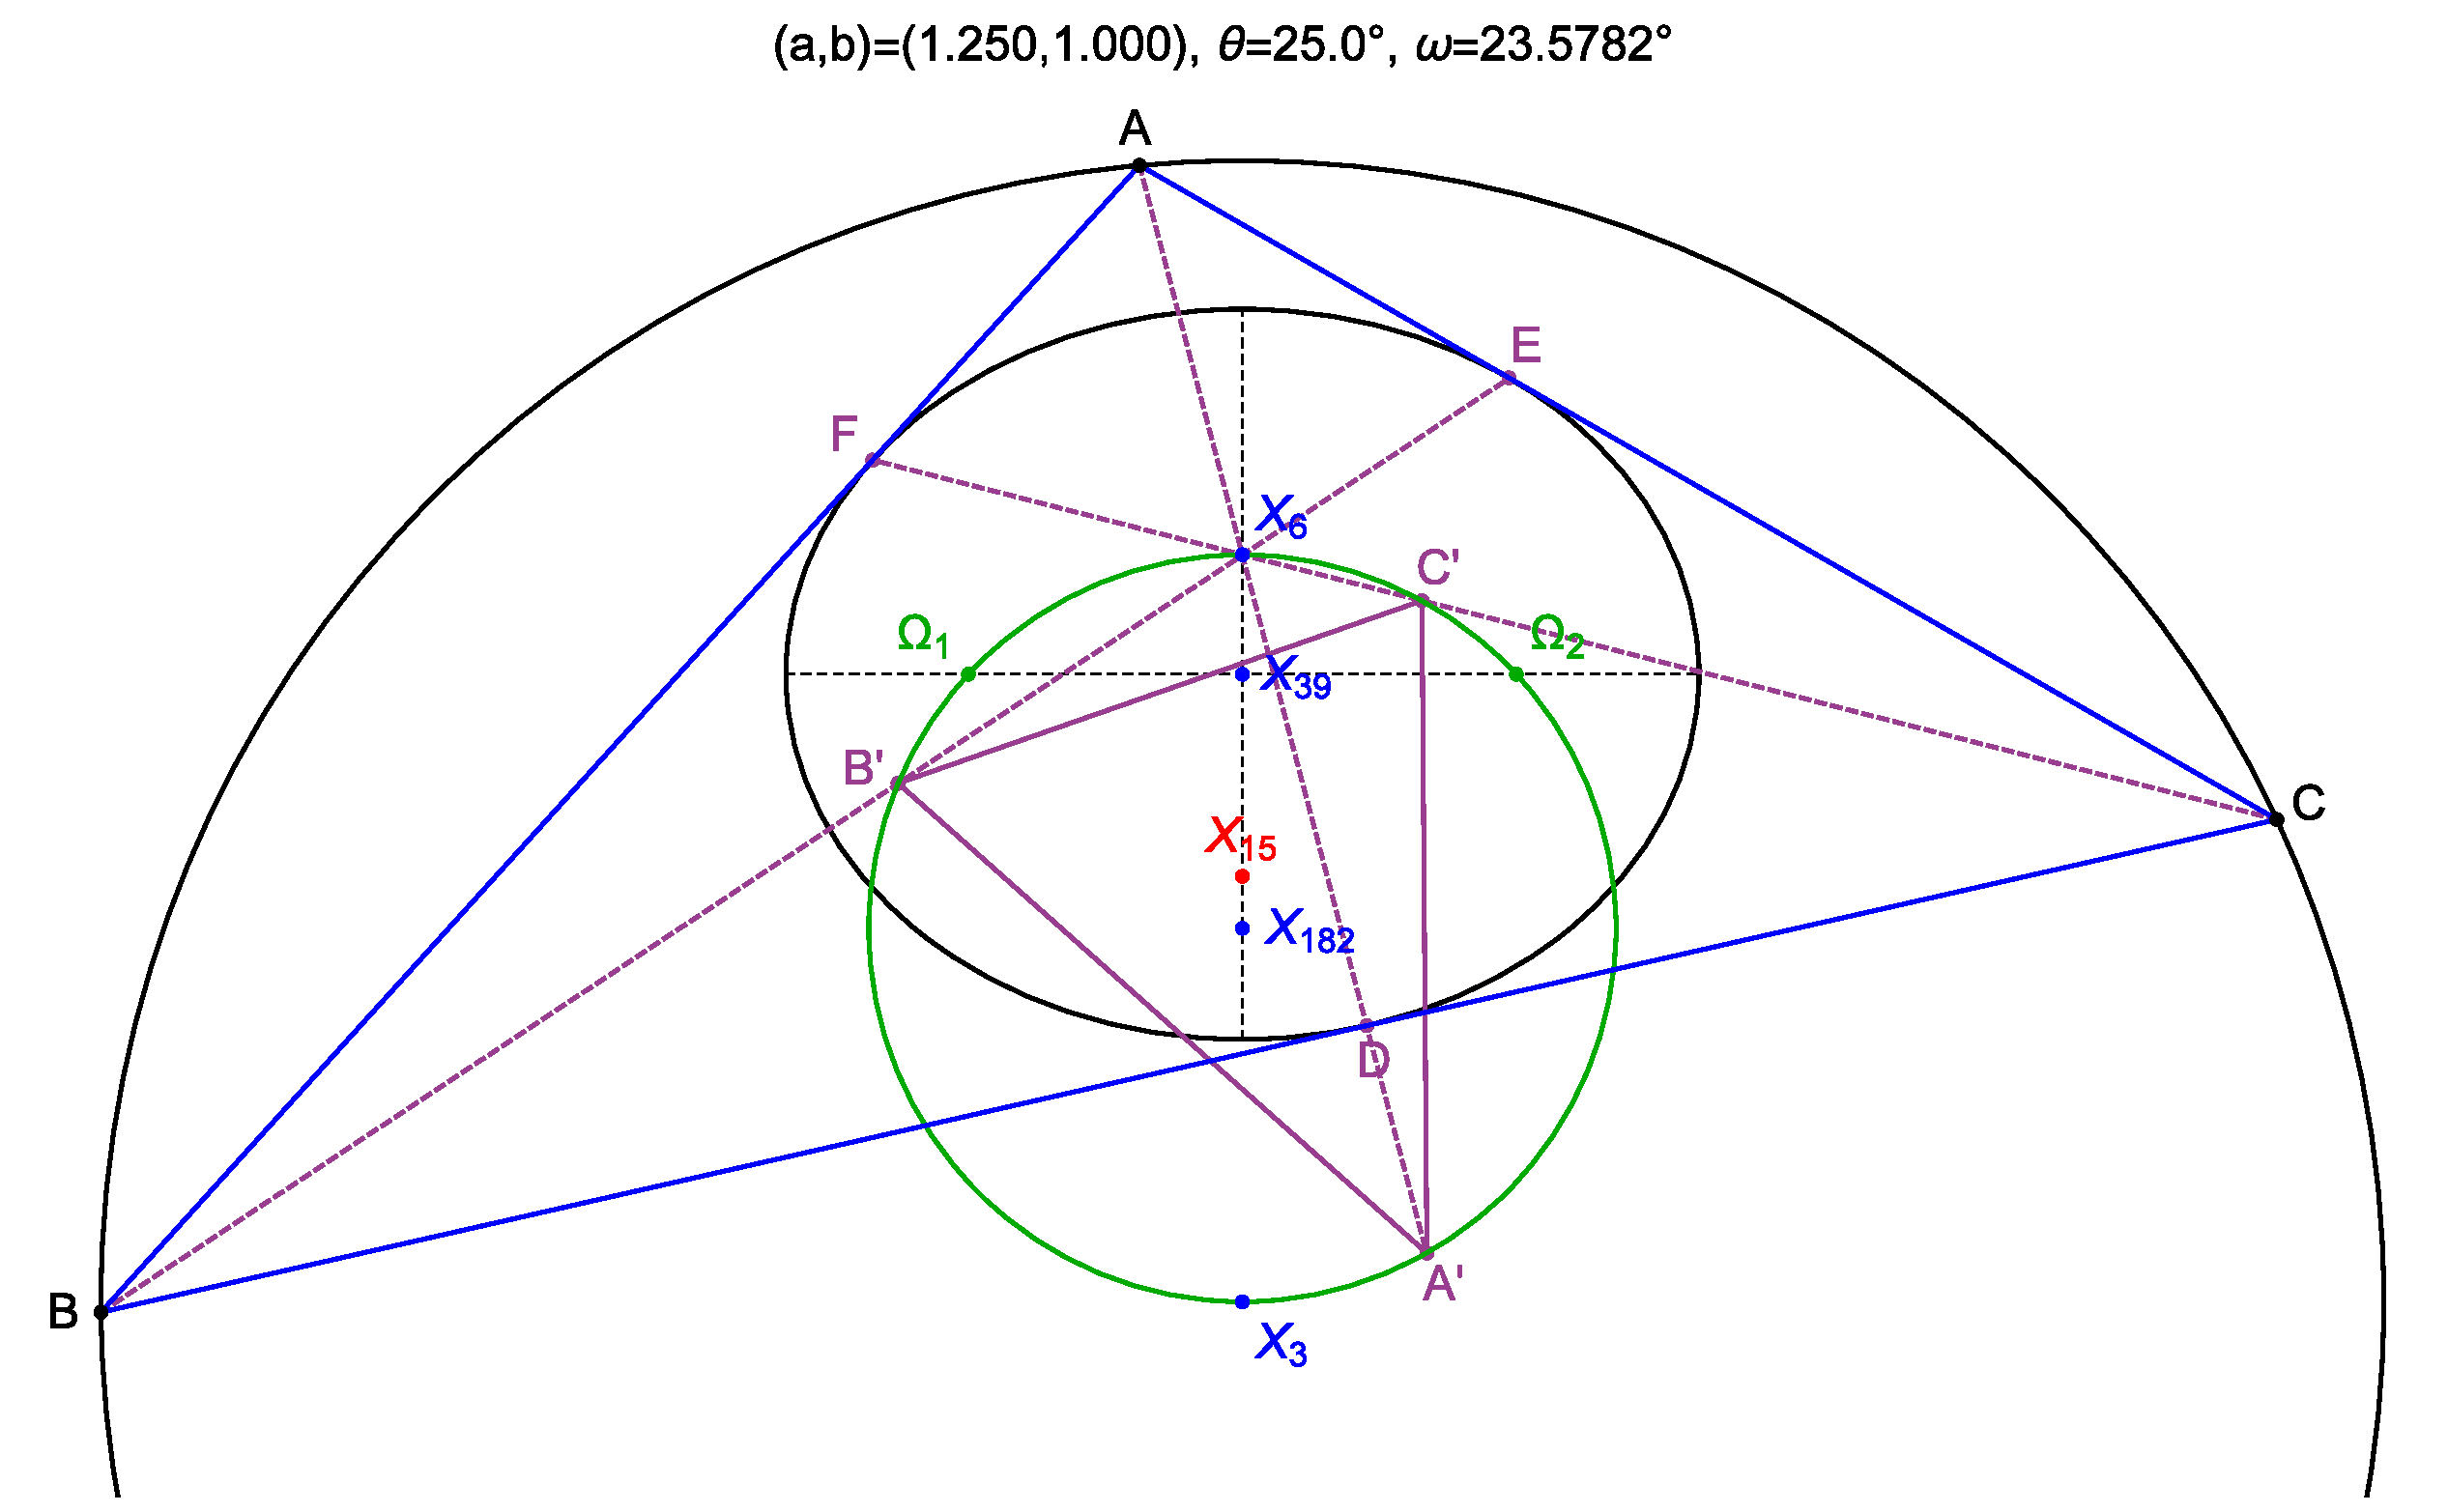
\includegraphics[width=\textwidth]{pics_06_0005_broc_porism_second_tri.eps}
    \caption{A Poncelet triangle (blue) $A B C$ in the Brocard Porism is shown inscribed in an external circle $\Gamma$ (black) and the Brocard inellipse $\E$ (black). The tangency points are given by intersections $D,E,F$ of symmedians (cevians through $X_6$) with the sidelengths. The Brocard points $\Omega_1$, $\Omega_2$ are stationary at the foci of $\E$. The Brocard circle $\K$ (green) contains $\Omega_1,\Omega_2$, the circumcenter $X_3$ and the symmedian point $X_6$, all of which are stationary. The center of $\K$ is $X_{182}$, the midpoint of $X_3 X_6$, aka the Brocard axis. Also shown (purple) is the second Brocard triangle $T'=A' B' C'$ inscribed in $\K$ whose vertices lie at the intersections of the symmedians with $\K$. Both isodynamic points $X_{15}$ and $X_{16}$ are on the Brocard axis and are stationary and common to both the original and the $T'$ family. \href{https://youtu.be/Wgwh4-neJp4}{Video}}
    \label{fig:broc-por-sec-tri}
\end{figure}

\begin{itemize}
   \item The $T'$ are Poncelet triangles of a second Brocard porism inscribed in $\K$ and circumscribed about a smaller, less eccentric ellipse $\E'$.
   \item Recursive calculation of $T'$ spawns an infinite sequence of ever-shrinking porisms which converge to the first isodynamic point $X_{15}$ \cite[Isodynamic Points]{mw}, common to all families. Successive Brocard points lie on two circular arcs.
   \item Recursive calculation of the {\em inverse} 2nd Brocard triangles (denoted $T^*$) converges to the segment between the so-called Beltrami points \cite{etc-bicentric}. 
   \item Sequential Brocard circles $\K,\K',\K'',...$ are nested within each other like a Russian doll.
   \item The discrete sequence of porisms is embedded in a continuous family where $T'$ (and its inverse) can be regarded as operators.
   \item The envelope of ellipses in the continuous porism is itself an ellipse with the isodynamic points as foci.
\end{itemize}

%\begin{figure}
%    \centering
%    \includegraphics[width=.6\textwidth]{pics/0015_matryoskha.png}
%    \caption{Nested Matryoshka/Babushka dolls (Russian: матрёшка, бабушка): similar to the infinite sequence of Brocard porisms and circles.}
%    \label{fig:matryoshka}
%\end{figure}

\subsection*{Related Work}

 A construction for the Brocard porism is given in \cite[Theorem 4.20, p. 129]{akopyan2007-conics}. In \cite[chapt XVII]{johnson1960} it is shown that a family of equilaterals embedded in a tilted plane projected to a fixed plane yields a  family of triangles with fixed Brocard angle, termed {\em equibrocardal}.
Bradley defines several conics associated to the Brocard porism \cite{bradley2011-brocard}. Odehnal has studied loci of triangle centers for the poristic triangle family \cite{odehnal2011-poristic} identifying dozens of stationary triangle centers; similarly, Pamfilos proves properties of the family of triangles with fixed 9-point and circumcircle \cite{pamfilos2020}.  We have previously studied triangle center loci over selected triangle families \cite{garcia2020-brocard,reznik2020-intelligencer}. We have also analyzed the Brocard porism alongside the Poncelet homothetic family establishing a similarity link between the two \cite{reznik2020-similarityII}.

%\subsection*{Article Structure} in Section~\ref{sec:review} we review definitions and prove basic Brocard relations required in further sections. In Section~\ref{sec:broc-second} we prove properties of the family of second Brocard triangles in a Brocard porism. In Section~\ref{sec:broc-second} we study the infinite, discrete sequence of porisms induced by iterative calculations of the second Brocard triangle. Finally, in Section~\ref{sec:continuous} we specify how said sequence is embedded in a continuous one.

%Appendix~\ref{app:isosceles} provides explicit expressions for the vertices of an isosceles triangle in the porism. Appendix~\ref{app:app_vertices} provides a 1d parametrization for any triangle in the porism. Appendix~\ref{app:app_further} contains additional supporting relations required by some of our proofs. Finally, Appendix~\ref{app:app_symbols} tabulates most symbols used herein.

\begin{figure}
    \centering
    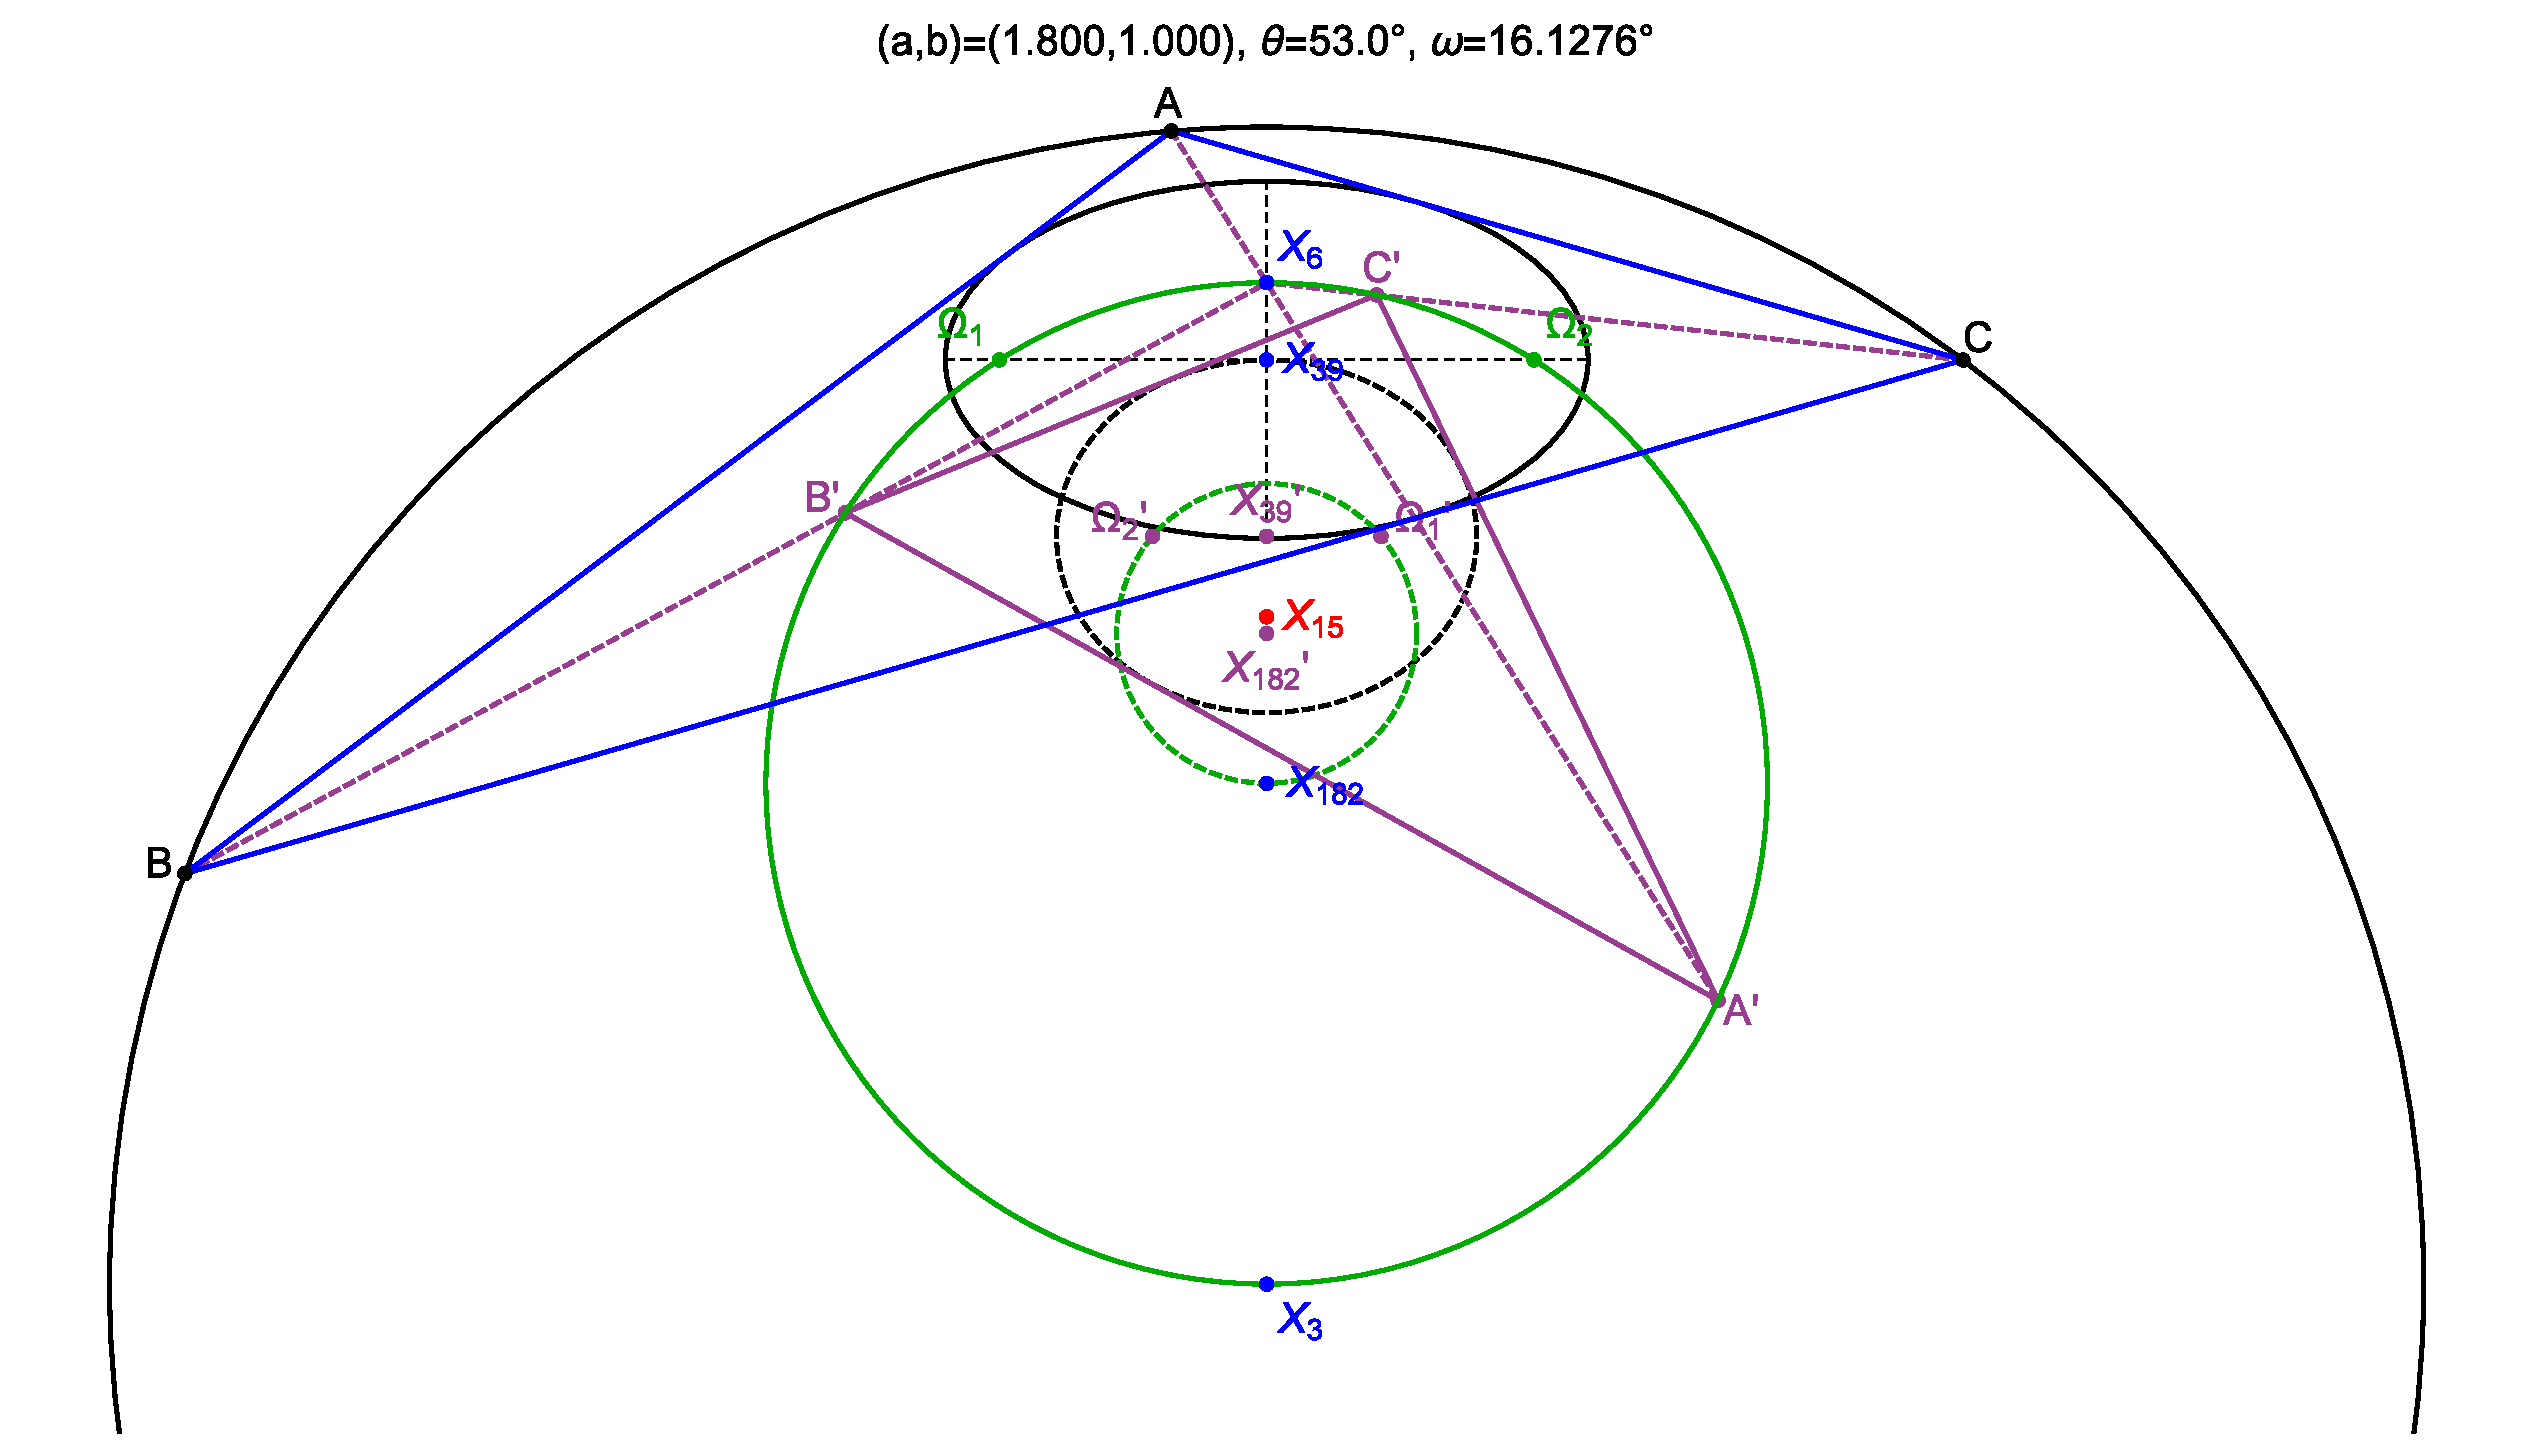
\includegraphics[width=\textwidth]{pics_06_0150_broc_porism_second_tri_iterate.eps}
    \caption{By construction (dashed purple), the second Brocard triangle $T'$ (purple), is inscribed in the Brocard circle $\K$ (green) of the its reference triangle $T$ (blue). Remarkably, over the Brocard porism (outer circle, inner ellipse, both in solid black), the Brocard points $\Omega_{2,1}'$ of $T'$ are also stationary. These coincide with the foci of a new, smaller, rounder, Brocard inellipse $\E'$ (dashed black). The new, stationary, Brocard circle $\K'$ (dashed green) is properly contained within $\K$. Notice the upper vertex of $\E'$ coincides with the Brocard midpoint $X_{39}$ of $T$. The isodynamic points $X_{15},X_{16}$ (latter not shown, above the page) are common and stationary for $T$ and $T'$. \href{https://youtu.be/MprJtB4UW9s}{Video}}
    \label{fig:iteration}
\end{figure}